Training the model with different sizes of latent dimensions yielded some different results, in different aspects of the tasks the model had. We can see how well the model performed on the different tasks in Table ~\ref{tab:cnn_results}\\

\begin{figure}[!ht]
  \centering
  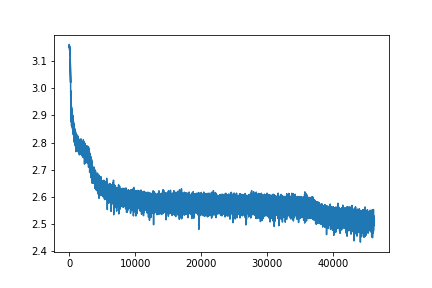
\includegraphics[width=0.4\linewidth]{latex/imgs/CNN_loss_latent_dimension_100.png}
  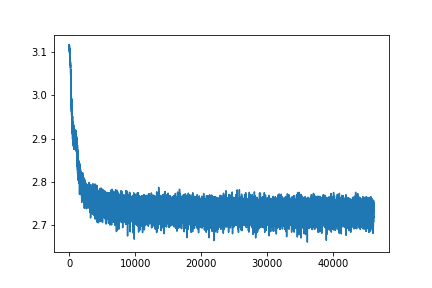
\includegraphics[width=0.4\linewidth]{latex/imgs/loss_latent_dimension_50.png}
  \caption{losses of the of cnn trained with latent dimension $4$x$100$(left) and $2$x$50$(right)}
  \label{fig:cnn_loss}
\end{figure}

\begin{table}[]
\begin{tabular}{|l|ll|ll|}
\hline
CNN Results & Final model                                  &                      & Minloss model                                &                      \\ \cline{2-5} 
            & \multicolumn{1}{l|}{Reconstruction accuracy} & Spearman correlation & \multicolumn{1}{l|}{Reconstruction accuracy} & Spearman correlation \\ \hline
4x100       & \multicolumn{1}{l|}{20.58\%}                 & 0.340                & \multicolumn{1}{l|}{20.39\%}                 & 0.145                \\ \hline
2x50        & \multicolumn{1}{l|}{14.69\%}                 & 0.351                & \multicolumn{1}{l|}{14.73\%}                 & 0.278                \\ \hline
\end{tabular}
\label{tab:cnn_results}
\end{table}


\begin{figure}[!ht]
  \centering
  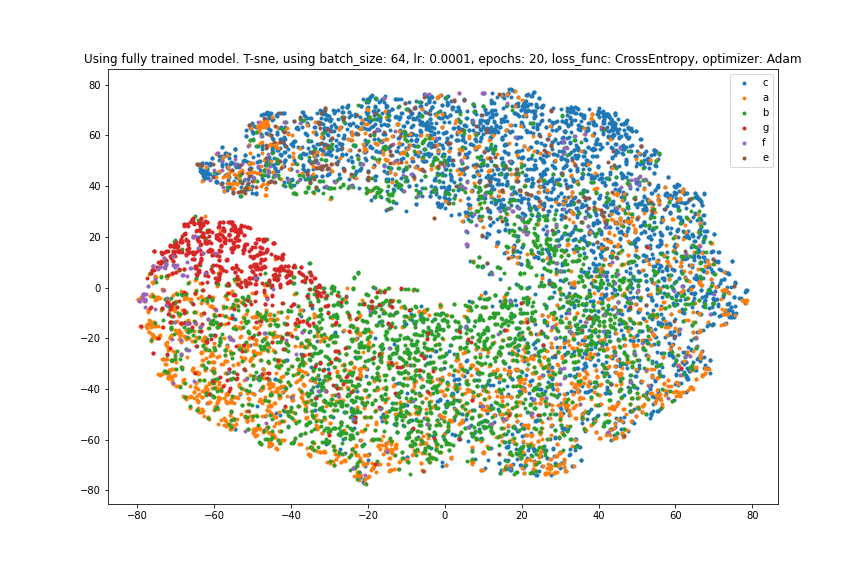
\includegraphics[width=0.4\linewidth]{latex/imgs/last_50.png}
  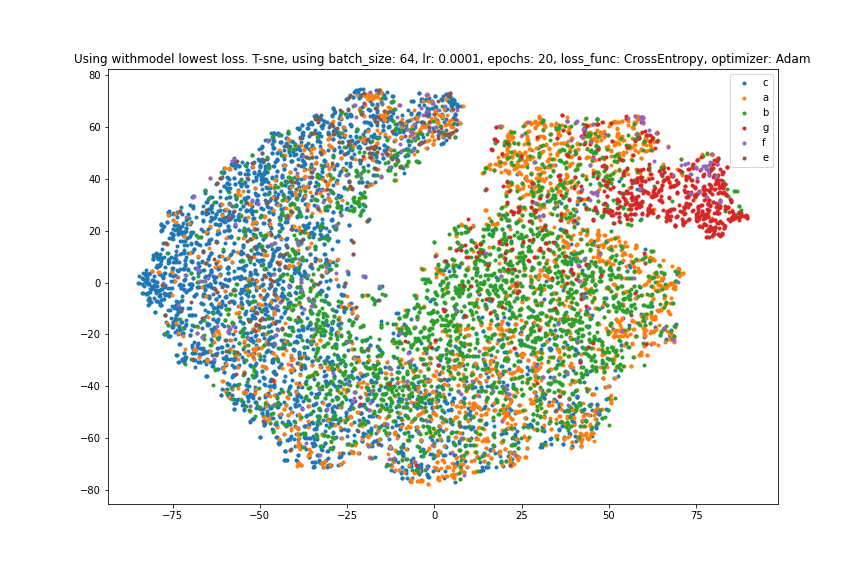
\includegraphics[width=0.4\linewidth]{latex/imgs/best_50.png}
  \caption{Plot showing secondary structure seperation with latent dimension $2$x$50$. Fully trained model(left), min loss model (left)}
  \label{fig:plot_50}
\end{figure}

\begin{figure}[!ht]
  \centering
  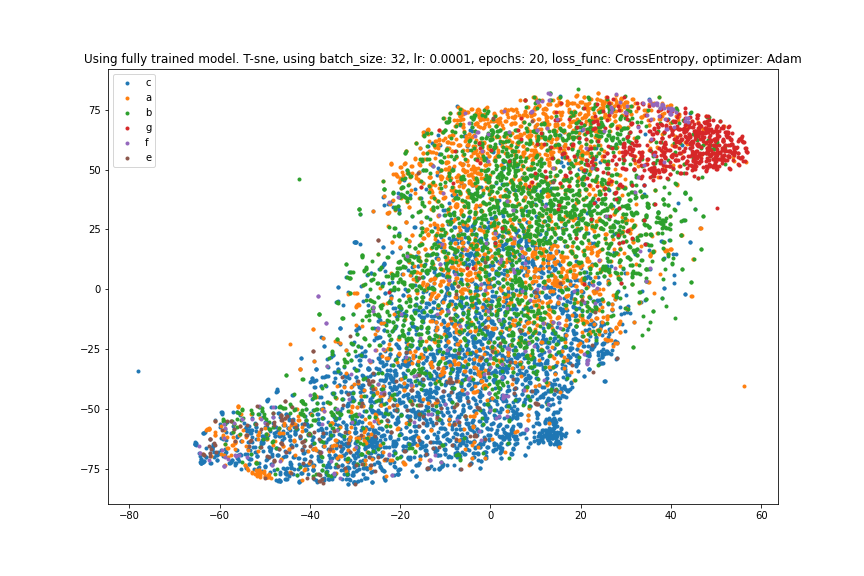
\includegraphics[width=0.4\linewidth]{latex/imgs/last_100.png}
  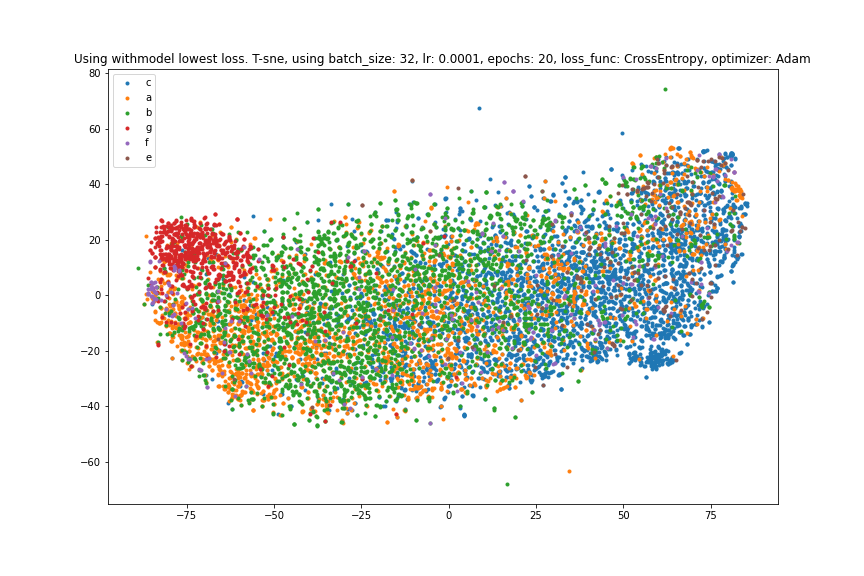
\includegraphics[width=0.4\linewidth]{latex/imgs/best_100.png}
  \caption{Plot showing secondary structure seperation with latent dimension $4$x$100$. Fully trained model(left), min loss model (left)}
  \label{fig:plot_100}
\end{figure}

\begin{figure}[!ht]
  \centering
  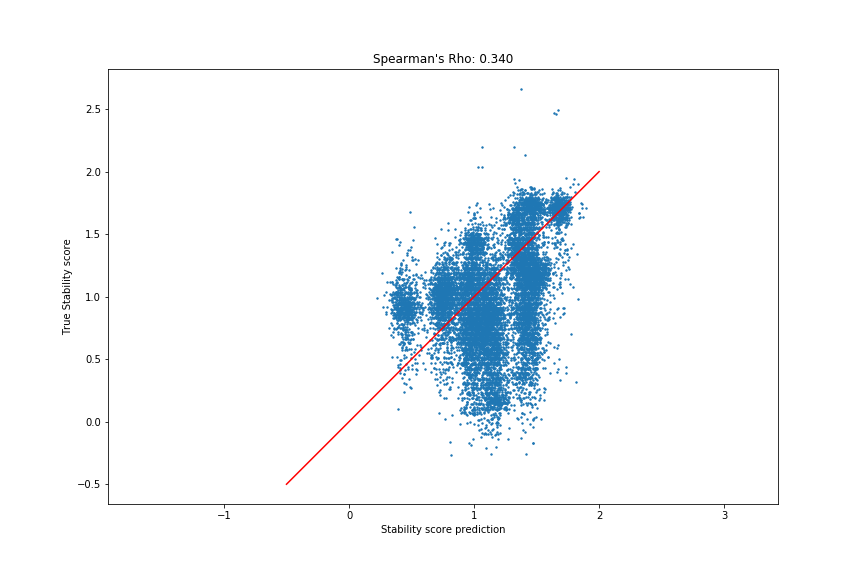
\includegraphics[width=0.4\linewidth]{latex/imgs/CNN_spearman_correlation_100_fully.png}
  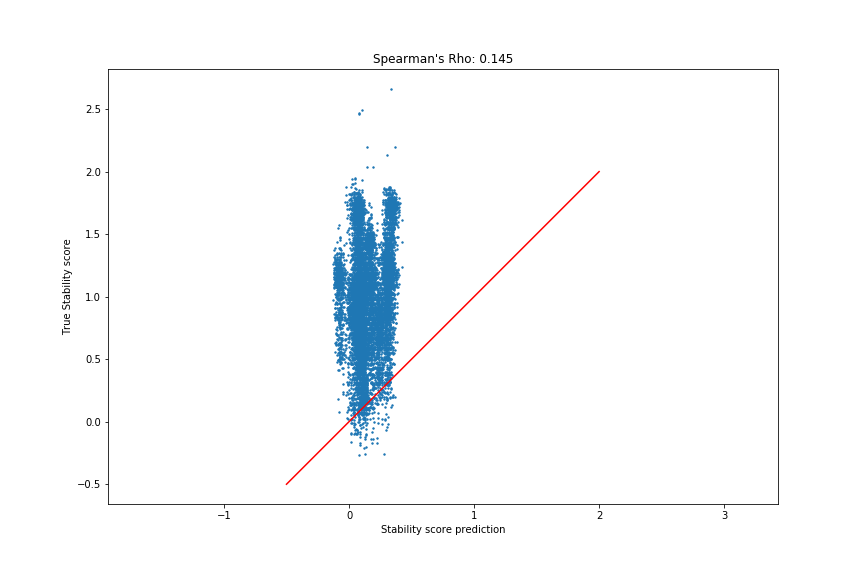
\includegraphics[width=0.4\linewidth]{latex/imgs/CNN_spearman_correlation_100_best.png}
  \caption{Graph showing the spearman correlation from model with latent dimension $4$x$100$. Fully trained model(left), min loss model (left)}
  \label{fig:stab_100}
\end{figure}

\begin{figure}[!ht]
  \centering
  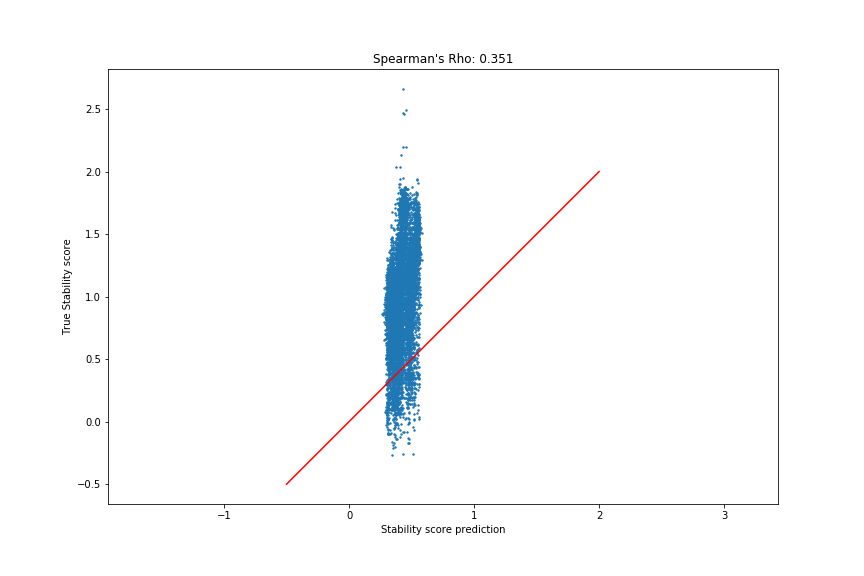
\includegraphics[width=0.4\linewidth]{latex/imgs/CNN_spearman_correlation_50_fully.png}
  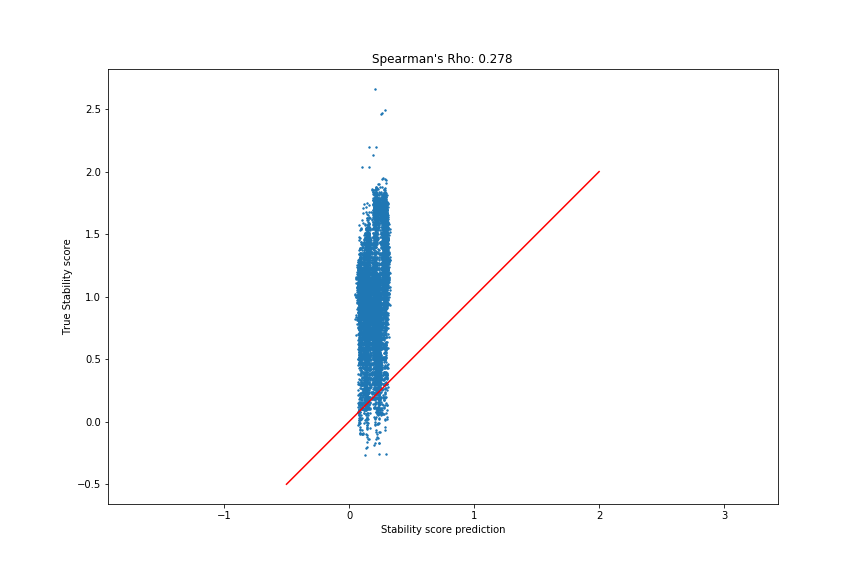
\includegraphics[width=0.4\linewidth]{latex/imgs/CNN_spearman_correlation_50_best.png}
  \caption{Graph showing the spearman correlation from model with latent dimension $2$x$50$. Fully trained model(left), min loss model (left)}
  \label{fig:stab_50}
\end{figure}